\section{Visualizers}
\subsection{LU Visualizer}
\subsubsection{Example 1: No arguments}{
\begin{lstlisting}[language=Python]
from BNumMet.Visualizers.LUVisualizer import LUVisualizer
luVisualizer = LUVisualizer()
display(luVisualizer.run())
\end{lstlisting}

\begin{enumerate}
  \item Initial State:\\  
    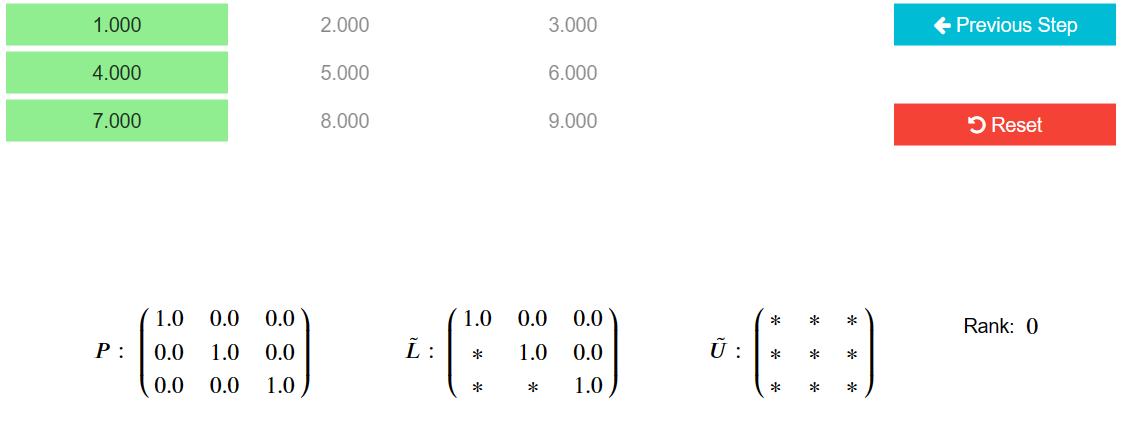
\includegraphics[scale=0.45]{Include/Images/Thesis/Documentation/Visualizers/LUVisualizer/Example 1/Example 1 - 00 - Initial State.png}
  \item Click on first column, second row:\\
    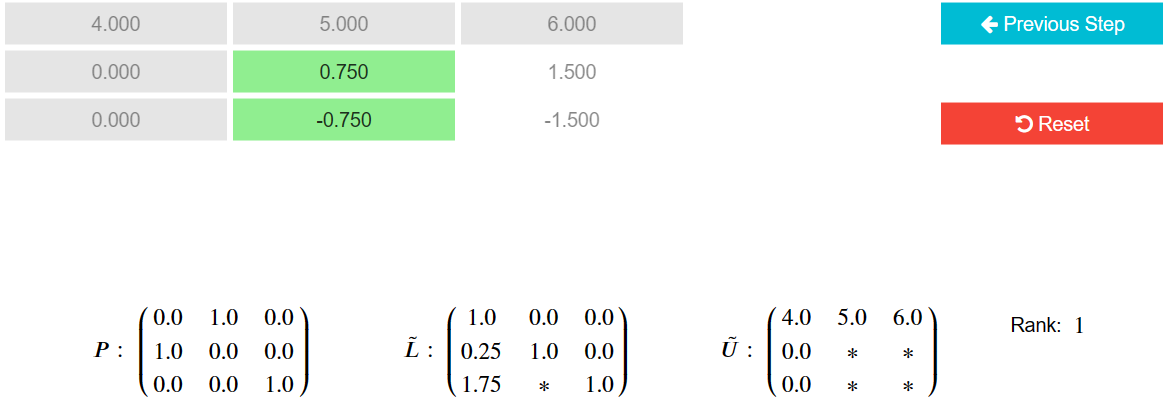
\includegraphics[scale=0.45]{Include/Images/Thesis/Documentation/Visualizers/LUVisualizer/Example 1/Example 1 - 01 - Click on 2 row.png}
  \item Click on second column, third row:\\
    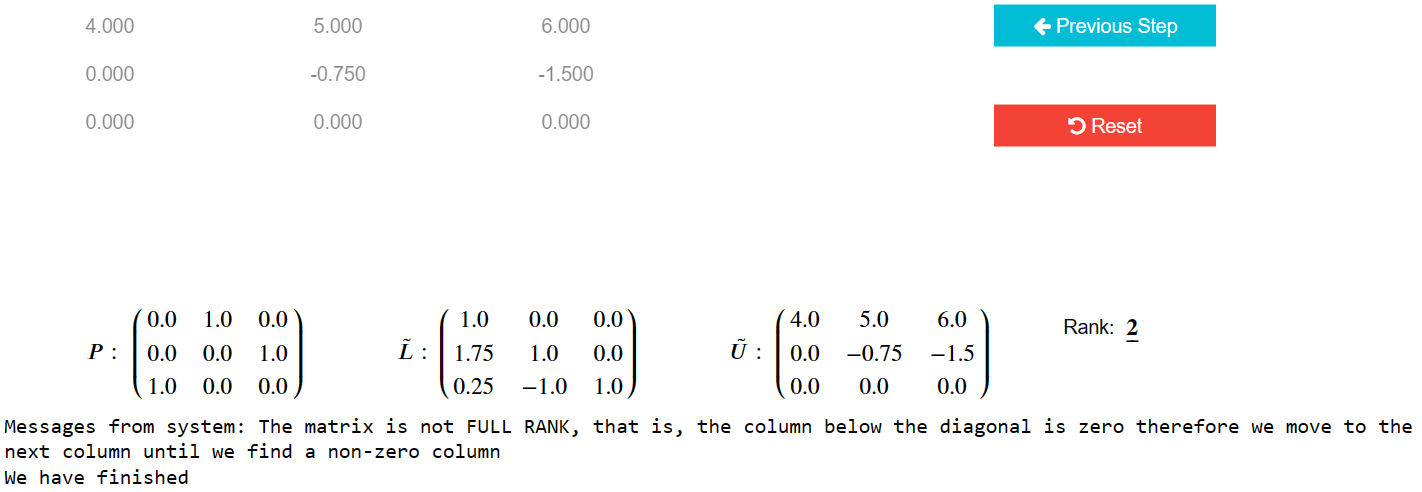
\includegraphics[scale=0.4]{Include/Images/Thesis/Documentation/Visualizers/LUVisualizer/Example 1/Example 1 - 02 - Click on 3 row.png}
  \item Click Previous Step:\\
    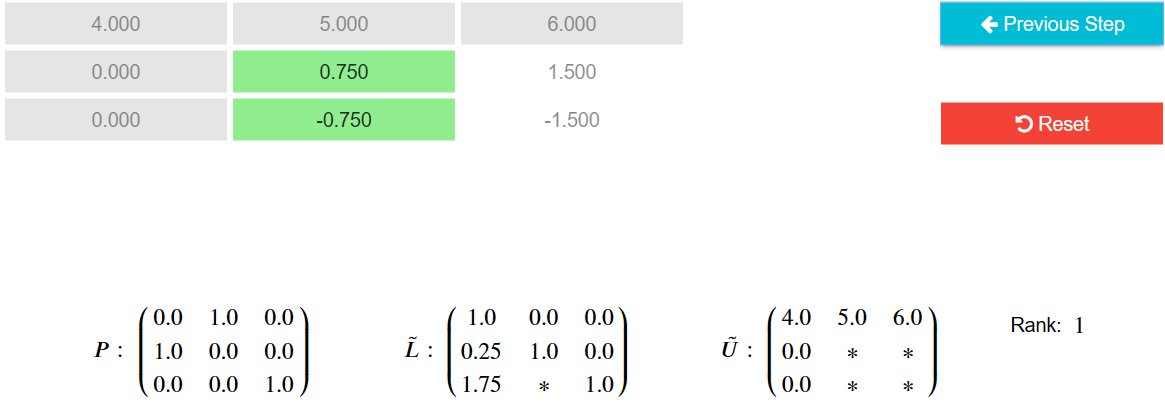
\includegraphics[scale=0.45]{Include/Images/Thesis/Documentation/Visualizers/LUVisualizer/Example 1/Example 1 - 03 - Click Previous Step.png}
  \item Click on second column, second row:\\
    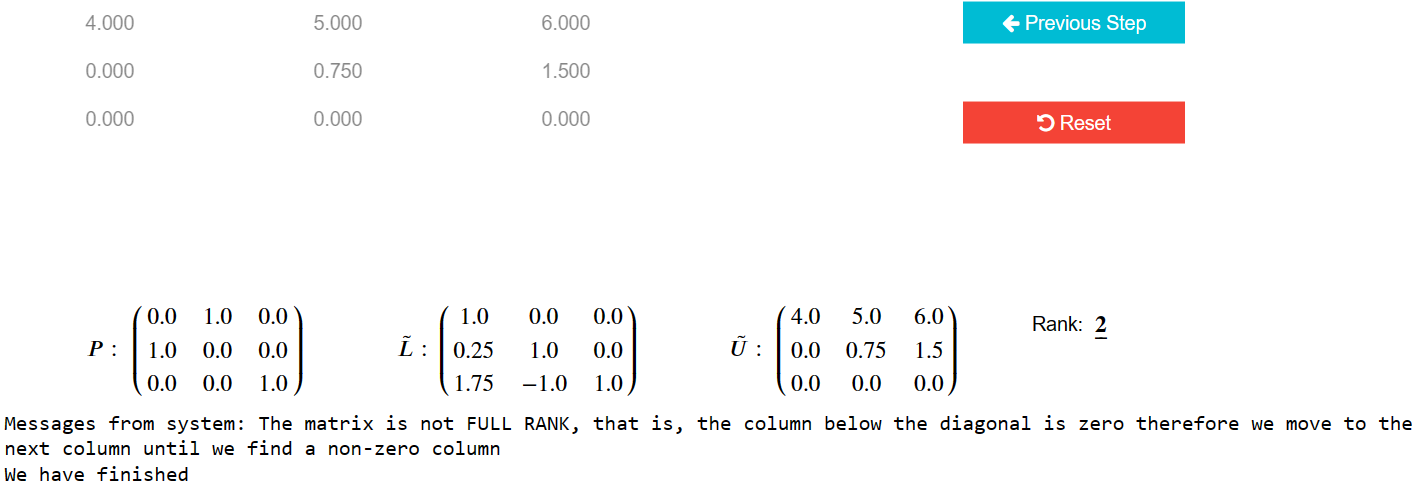
\includegraphics[scale=0.4]{Include/Images/Thesis/Documentation/Visualizers/LUVisualizer/Example 1/Example 1 - 04. - Click on 2 row.png}
  \item Click on Reset\\
      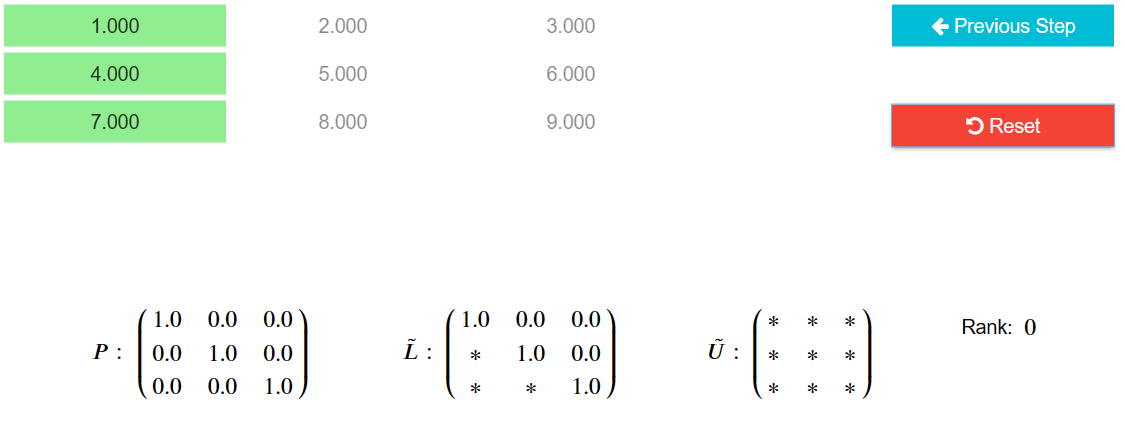
\includegraphics[scale=0.45]{Include/Images/Thesis/Documentation/Visualizers/LUVisualizer/Example 1/Example 1 - 05 - Click on Reset.png}
\end{enumerate}
}
\subsubsection{Example 2: Arguments and Rank Revealing}{
\begin{lstlisting}[language=Python]
from BNumMet.Visualizers.LUVisualizer import LUVisualizer
A = np.array([[1,2,3,7], [1,2,3,7], [1,2,3,7],[1,2,4,7]], dtype=float)
luVisualizer = LUVisualizer(A)
display(luVisualizer.run())
\end{lstlisting}

\begin{enumerate}
\item Initial State: \\
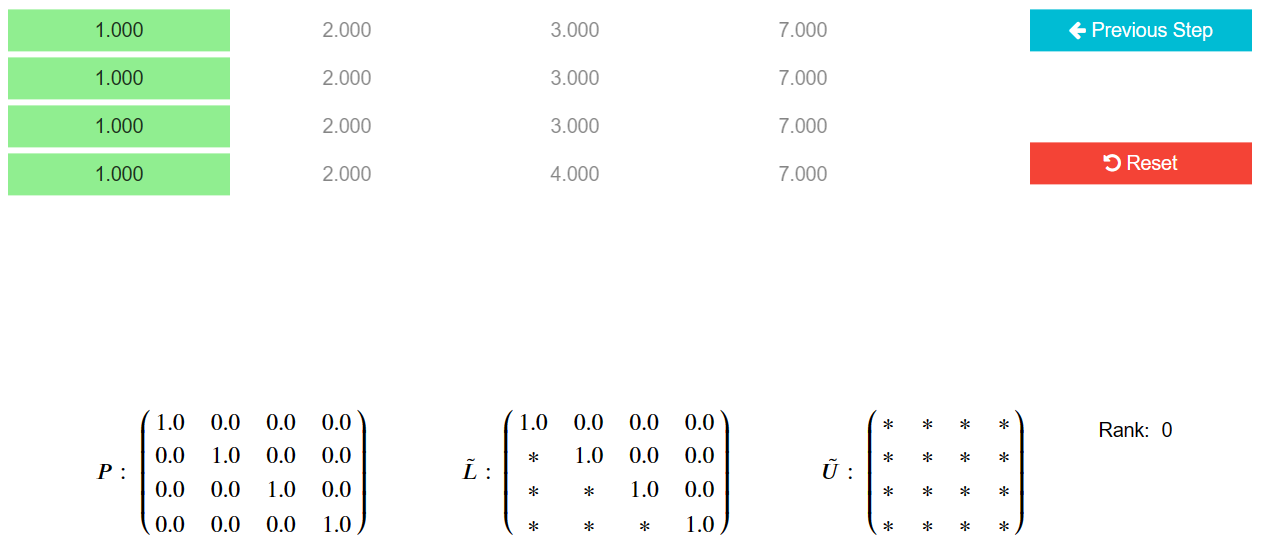
\includegraphics[scale=0.45]{Include/Images/Thesis/Documentation/Visualizers/LUVisualizer/Example 2/Example 2 - 00 - Initial State.png}

\item Click on the first column, second row: \\
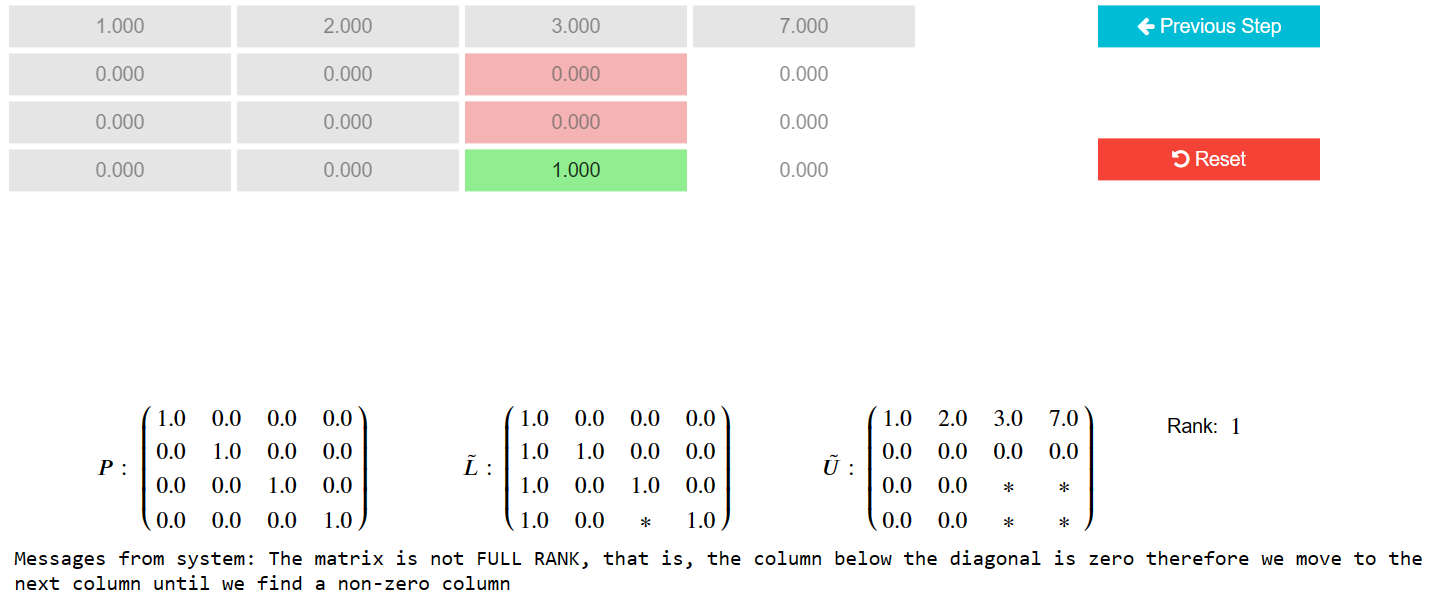
\includegraphics[scale=0.4]{Include/Images/Thesis/Documentation/Visualizers/LUVisualizer/Example 2/Example 2 - 01 - Click first column, second row.png}

\item Click on the third column, fourth row: \\
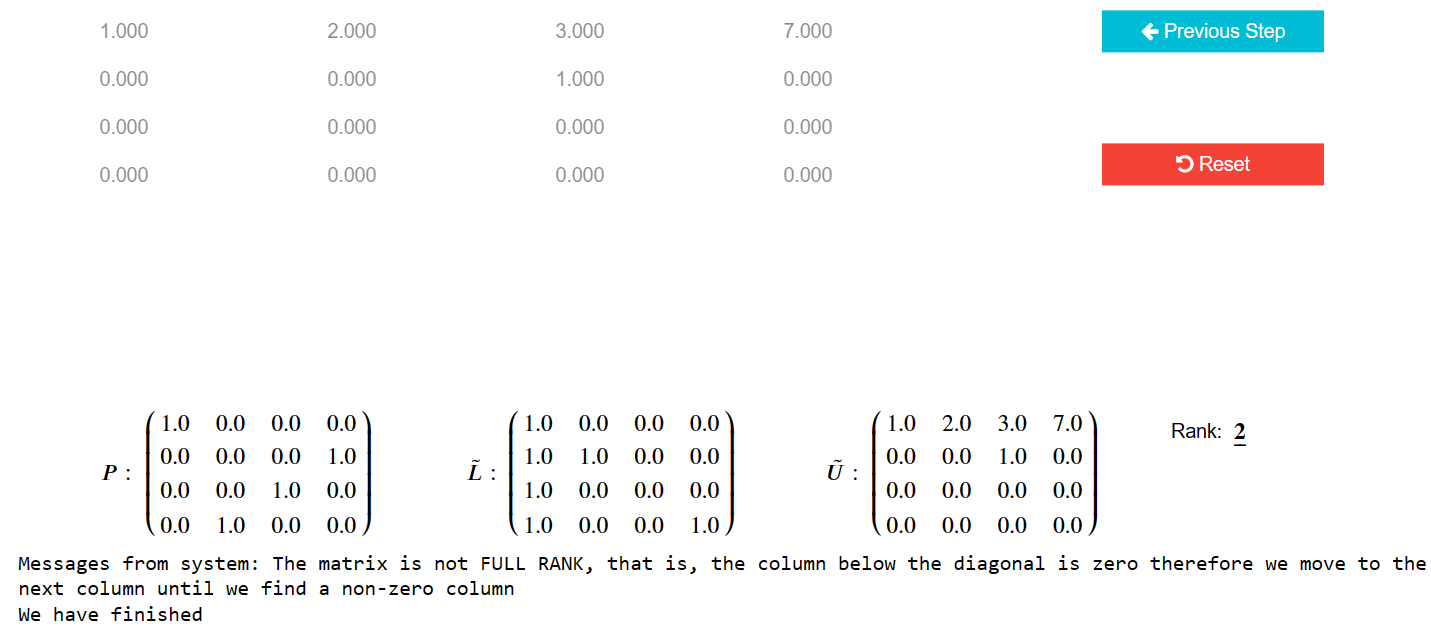
\includegraphics[scale=0.4]{Include/Images/Thesis/Documentation/Visualizers/LUVisualizer/Example 2/Example 2 - 02 - Click thirdcolumn, fourth row.png}
\end{enumerate}
}


\subsection{Interpolation Visualizer}
\subsubsection{Example 1}
\begin{lstlisting}[language=Python]
from BNumMet.Visualizers.InterpolationVisualizer import InterpolVisualizer
interpolVisualizer = InterpolVisualizer()
display(interpolVisualizer.run())
\end{lstlisting}
\begin{enumerate}
\item Initial State: \\
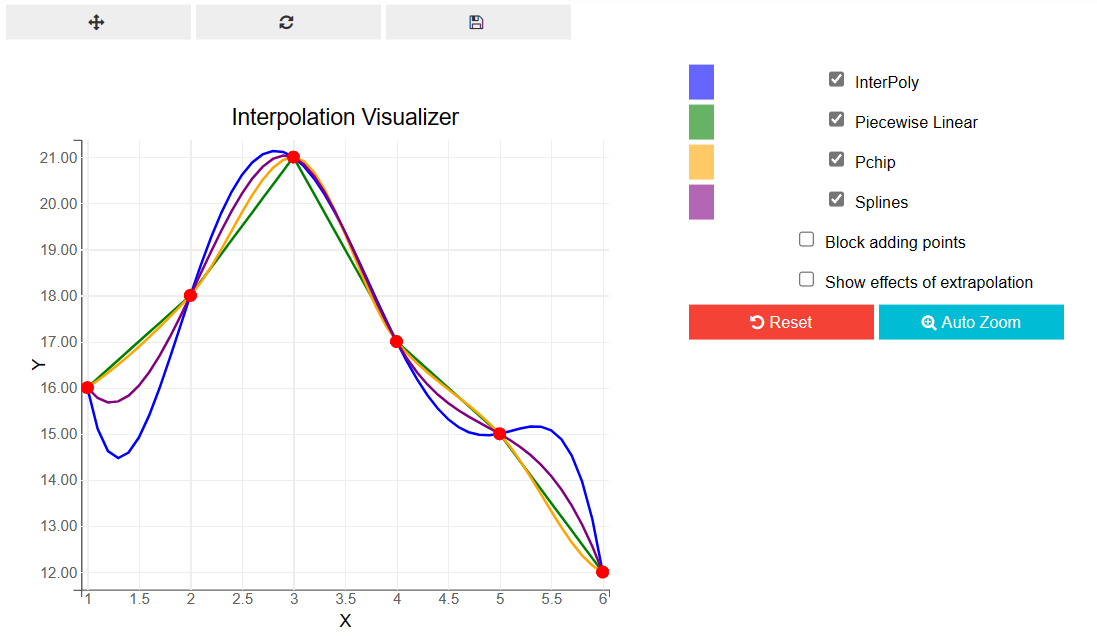
\includegraphics[scale=0.5]{Include/Images/Thesis/Documentation/Visualizers/Interpolation/Example 1/Example 1 - 00 - Initial State.png}

\item Checked Box Extrapolation and AutoZoom: \\
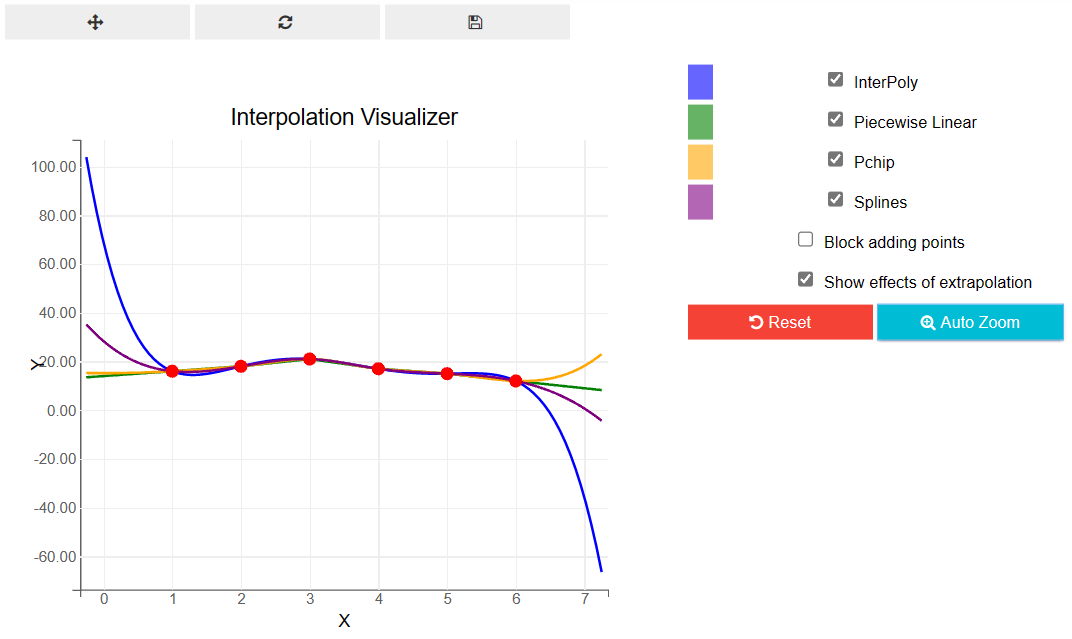
\includegraphics[scale=0.5]{Include/Images/Thesis/Documentation/Visualizers/Interpolation/Example 1/Example 1 - 01 - Checked Box Extrapolation and AutoZoom.png}

\item Reset Button: \\
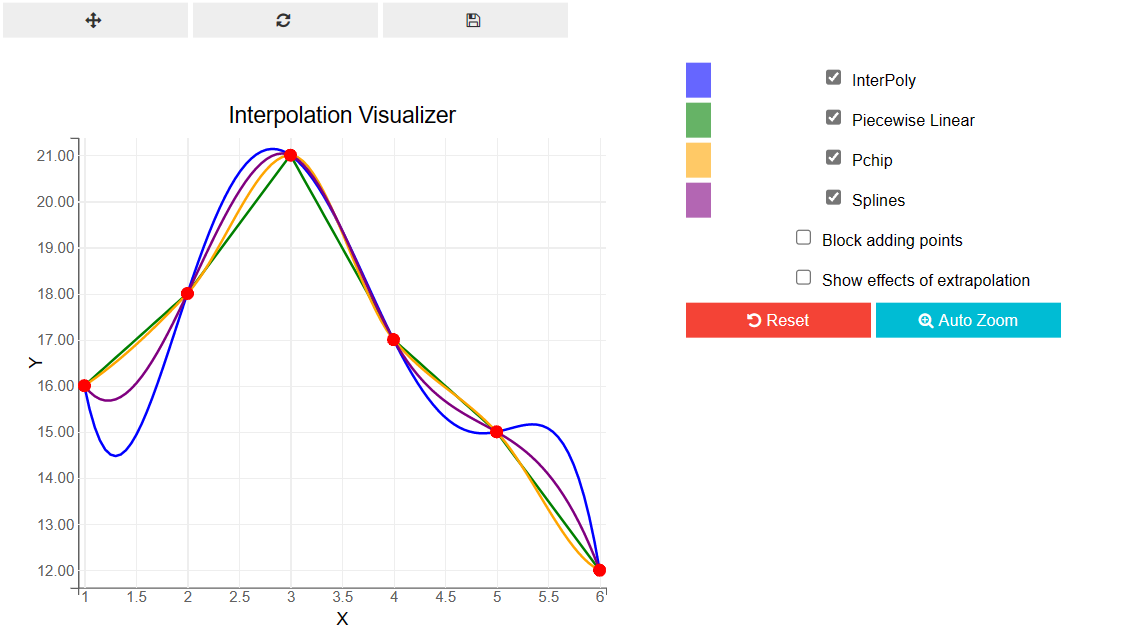
\includegraphics[scale=0.5]{Include/Images/Thesis/Documentation/Visualizers/Interpolation/Example 1/Example 1 - 02 - Reset Button.png}

\item Added Point: \\
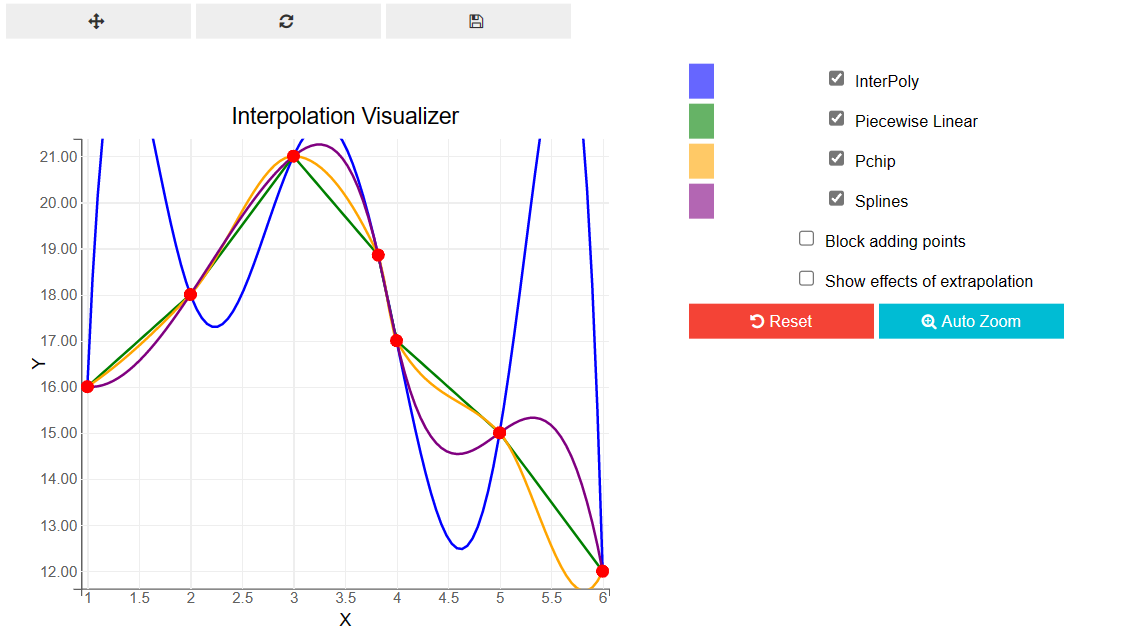
\includegraphics[scale=0.5]{Include/Images/Thesis/Documentation/Visualizers/Interpolation/Example 1/Example 1 - 03 - Added Point.png}

\item AutoZoom: \\
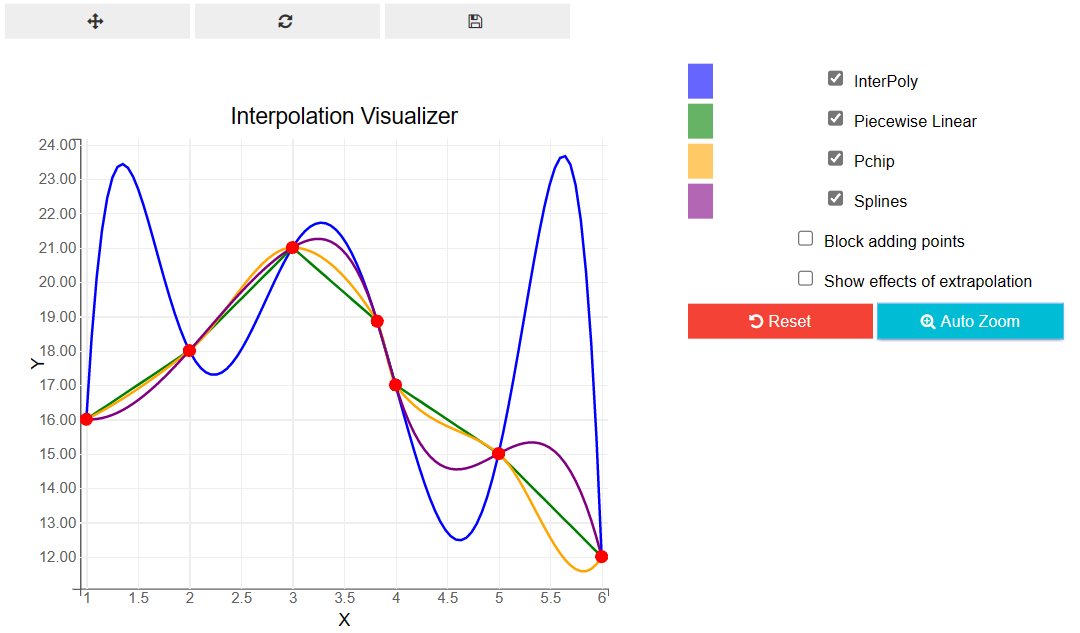
\includegraphics[scale=0.5]{Include/Images/Thesis/Documentation/Visualizers/Interpolation/Example 1/Example 1 - 04 -AutoZoom.png}
\end{enumerate}

\subsection{NonLinear Visualizer}
\subsubsection{Example 1: No arguments}
\begin{lstlisting}[language=Python]
from BNumMet.Visualizers.NonLinearVisualizer import NonLinearVisualizer
zerosVisualizer = NonLinearVisualizer()
zerosVisualizer.run()
\end{lstlisting}
\begin{enumerate}
    \item Initial State\\
    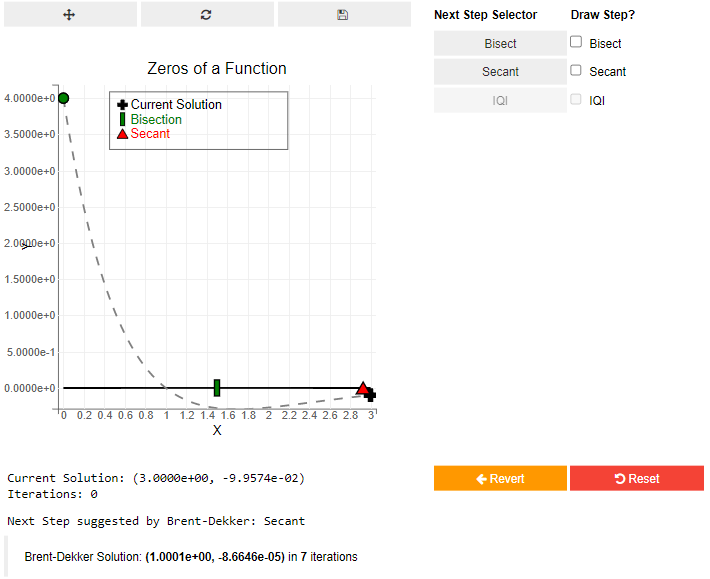
\includegraphics[scale=0.6]{Include/Images/Thesis/Documentation/Visualizers/NonLinear/Example 1/Example 1 - 00 - Initial State.png}
    \item Click on bisection checkbox\\
    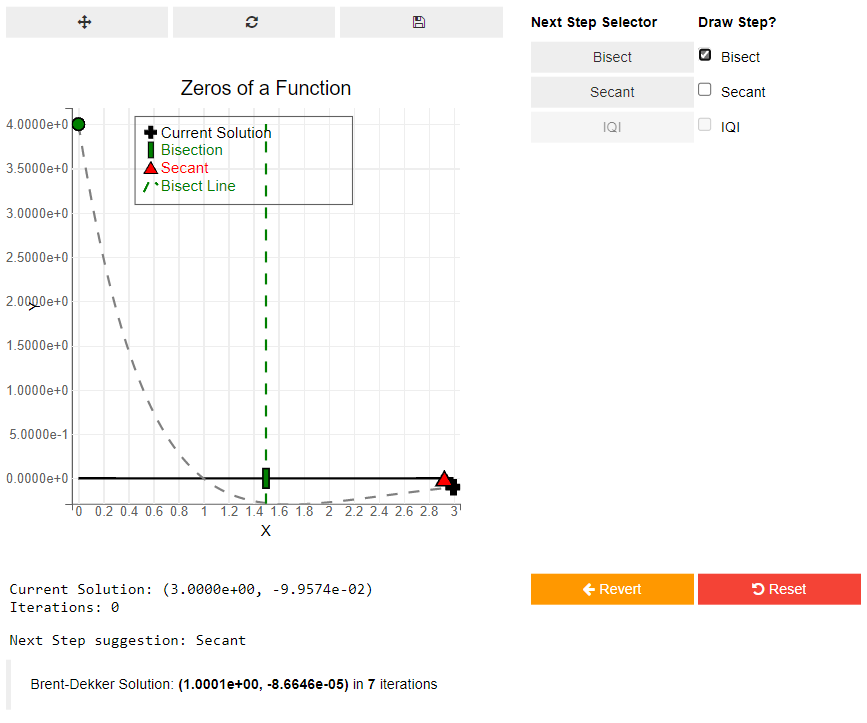
\includegraphics[scale=0.6]{Include/Images/Thesis/Documentation/Visualizers/NonLinear/Example 1/Example 1 - 01 - Bisection Checkbox.png}
    \item Click Secant Button\\
    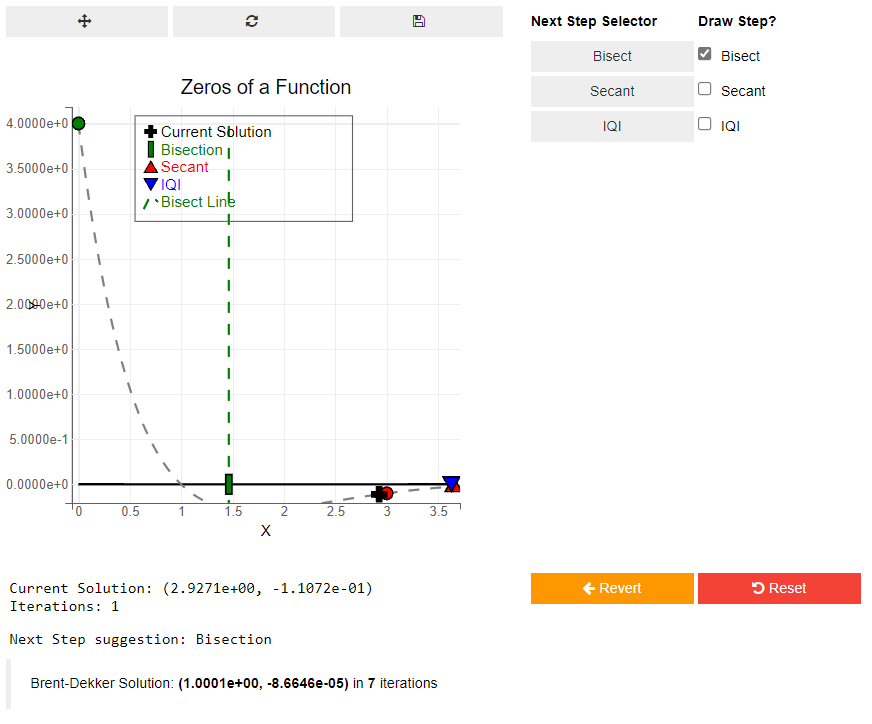
\includegraphics[scale=0.6]{Include/Images/Thesis/Documentation/Visualizers/NonLinear/Example 1/Example 1 - 02 - Click Secant.png}
    \item Some iterations after with secant checkbox clicked\\
    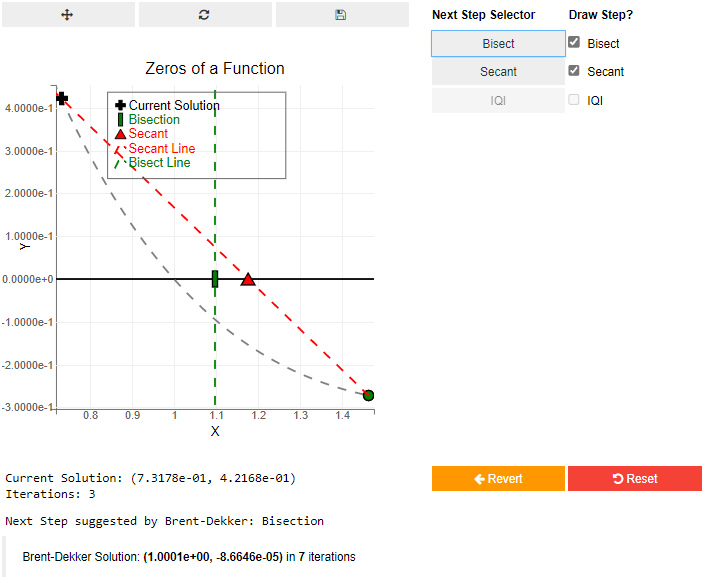
\includegraphics[scale=0.6]{Include/Images/Thesis/Documentation/Visualizers/NonLinear/Example 1/Example 1 - 03 - SOme iterations with secant checkbox.png}
    \item IQI Checkbox Only\\
    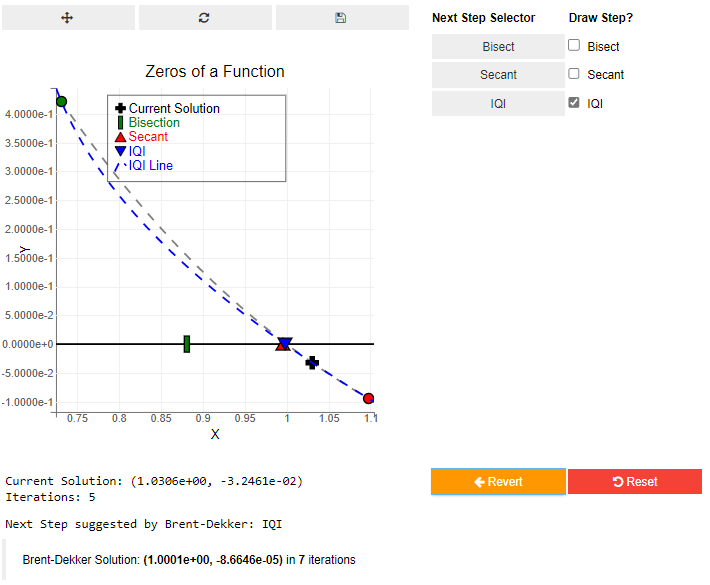
\includegraphics[scale=0.6]{Include/Images/Thesis/Documentation/Visualizers/NonLinear/Example 1/Example 1 - 04 - IQI checkbox only.png}
\end{enumerate}



\subsubsection{Example 2: With Arguments}
\begin{lstlisting}[language=Python]
from BNumMet.Visualizers.NonLinearVisualizer import NonLinearVisualizer
f2 = lambda x: 0 if abs(x) < 3.8 * 10 ** (-4) else float(x * np.exp(-1 / x**2))
interval = (-1, 2)
zerosVisualizer = NonLinearVisualizer(f2,interval)
zerosVisualizer.run()
\end{lstlisting}

\begin{enumerate}
    \item Initial State\\
    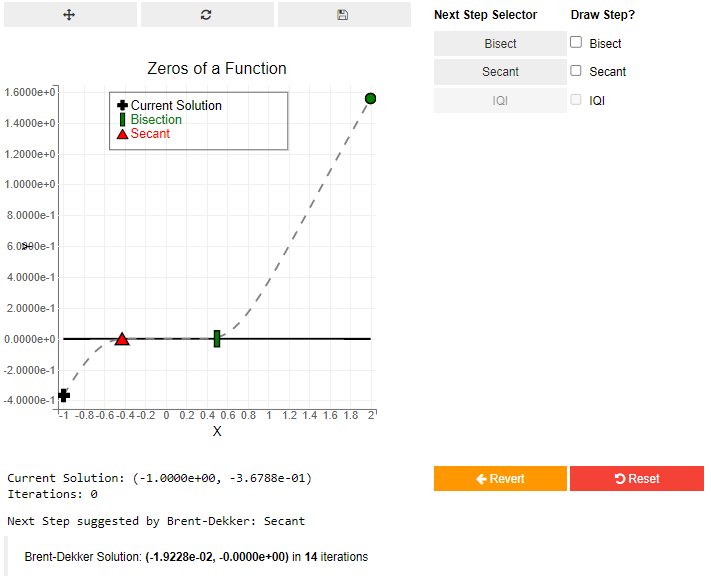
\includegraphics[scale=0.6]{Include/Images/Thesis/Documentation/Visualizers/NonLinear/Example 2/Example 2 - 00 - Initial State.png}
    \item All Checkboxes checked\\
    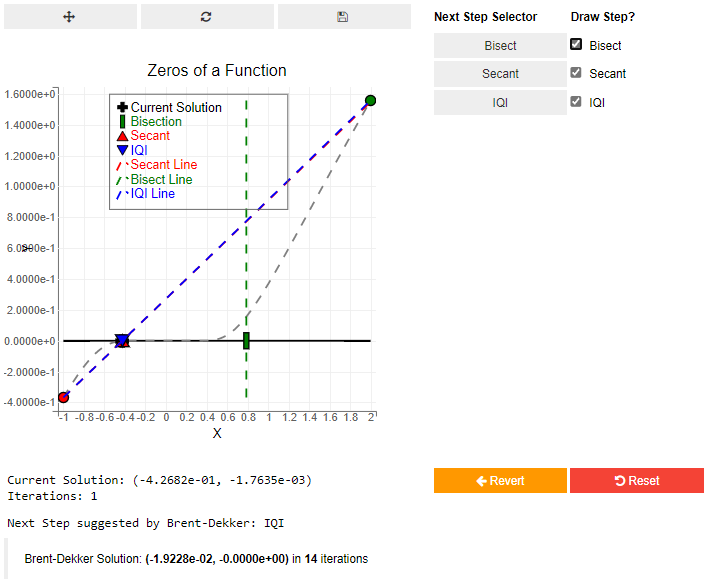
\includegraphics[scale=0.6]{Include/Images/Thesis/Documentation/Visualizers/NonLinear/Example 2/Example 2 - 01 - All Check Boxes.png}
    \item Click secant and click select all checkboxes again\\
    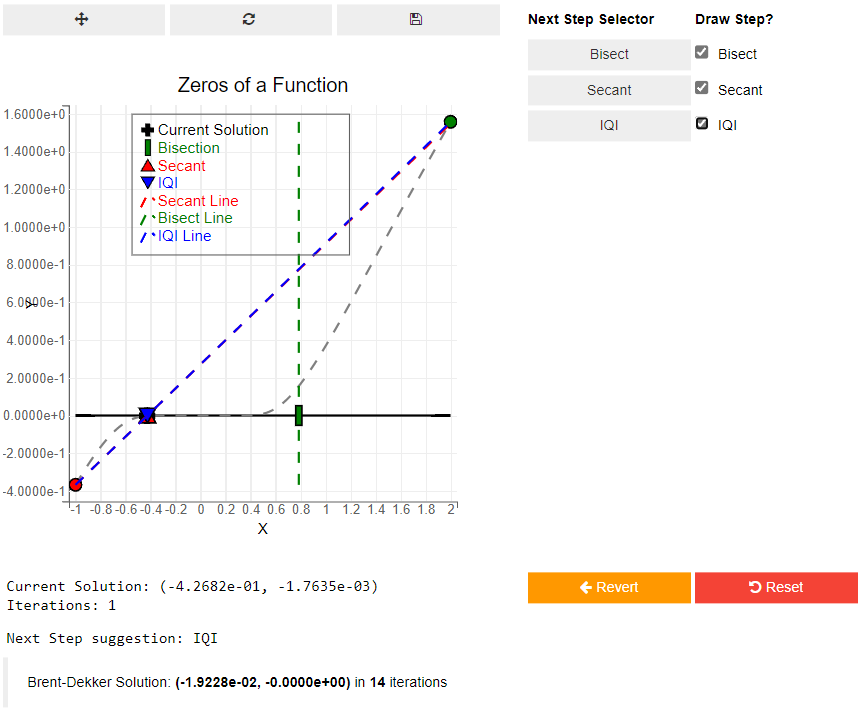
\includegraphics[scale=0.6]{Include/Images/Thesis/Documentation/Visualizers/NonLinear/Example 2/Example 2 - 02 - Click secant and All Check Boxes.png}
    \item Revert Button\\
    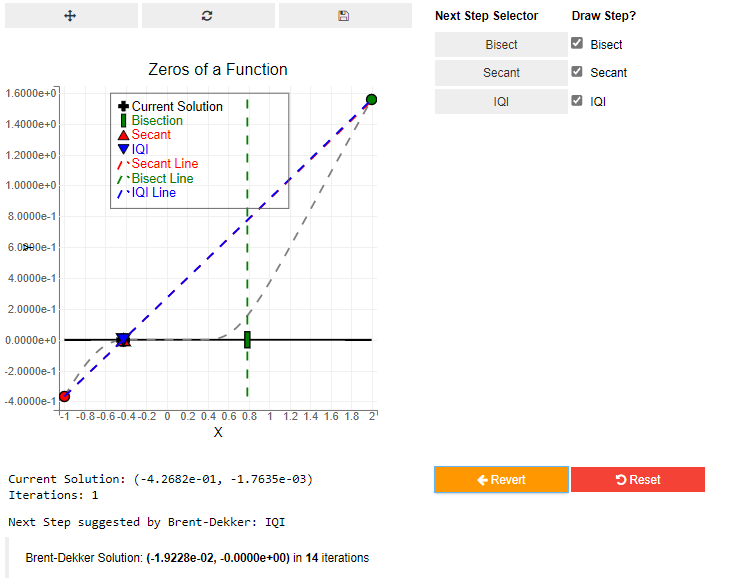
\includegraphics[scale=0.6]{Include/Images/Thesis/Documentation/Visualizers/NonLinear/Example 2/Example 2 - 03 - Revert Button.png}
    \item Some iterations\\
    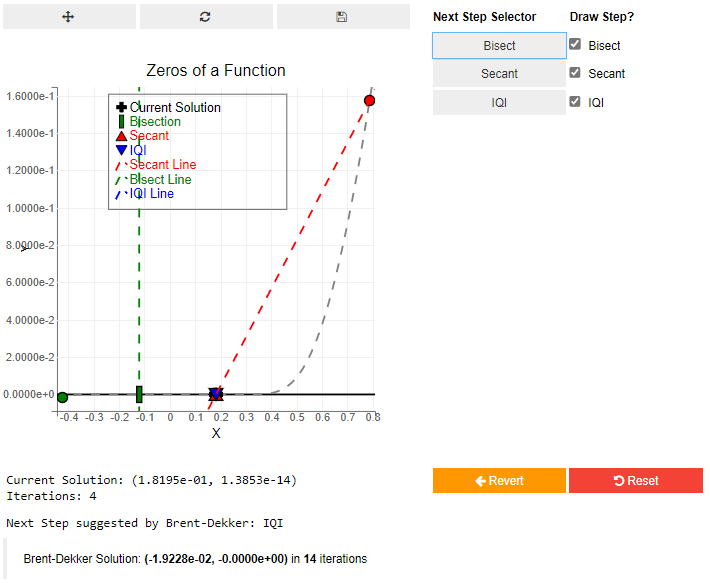
\includegraphics[scale=0.6]{Include/Images/Thesis/Documentation/Visualizers/NonLinear/Example 2/Example 2 - 04 - Some Iterations.png}
    \item Reset Button clicked\\
    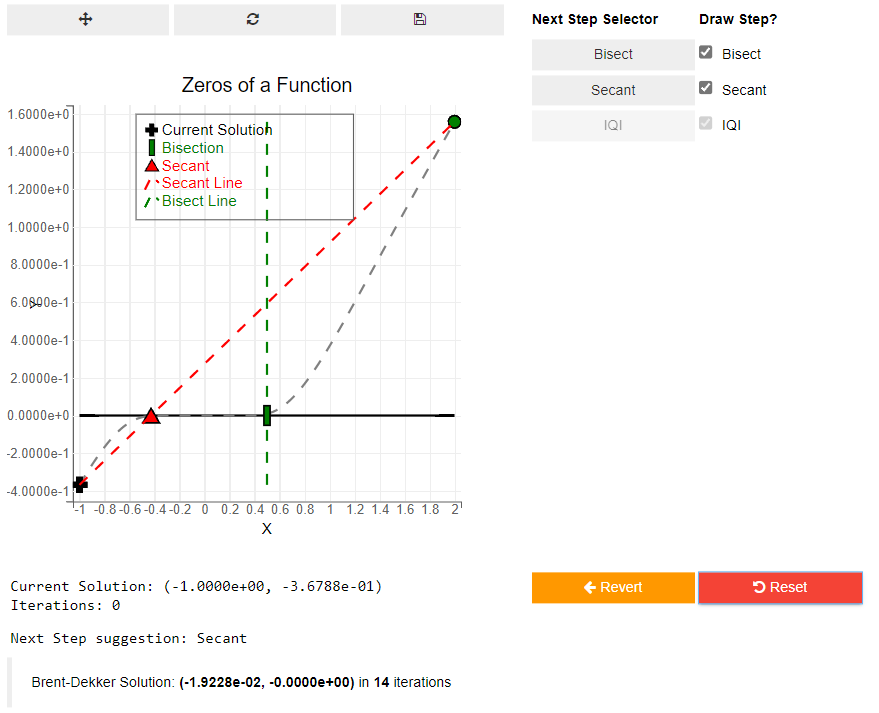
\includegraphics[scale=0.6]{Include/Images/Thesis/Documentation/Visualizers/NonLinear/Example 2/Example 2 - 04 - Reset Button.png}
\end{enumerate}





\subsection{Least Squares Visualizer}
\subsubsection{Example 1: Polynomial Fit of Varying degree}{
\begin{lstlisting}[language=Python]
from BNumMet.Visualizers.LeastSquaresVisualizer import LSPVisualizer
xData = np.array([0, 1, 2, 3, 4, 5])
yData = np.array([4.5, 2.4, 1.5, 1, 1.5, 2.4])
lspVisualizer = LSPVisualizer(xData, yData)
lspVisualizer.run()
\end{lstlisting}

\begin{enumerate}
    \item Initial State\\
    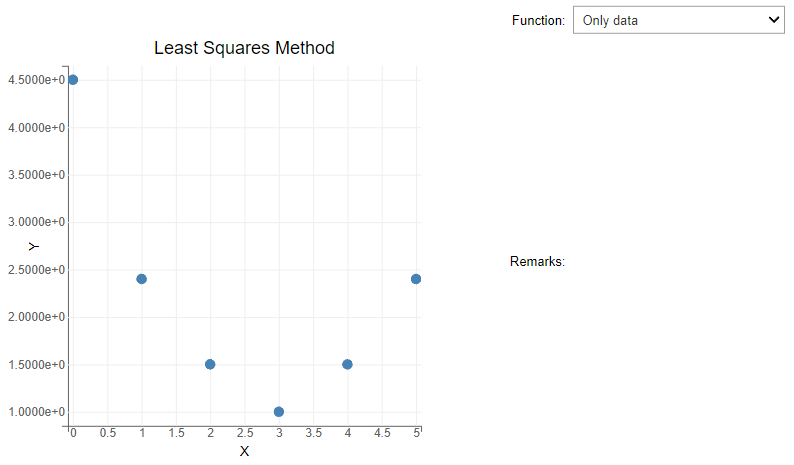
\includegraphics[scale=0.6]{Include/Images/Thesis/Documentation/Visualizers/LeastSquares/Example 1/Example 1 - 00 - Initial State.png}
    \item Selector\\
    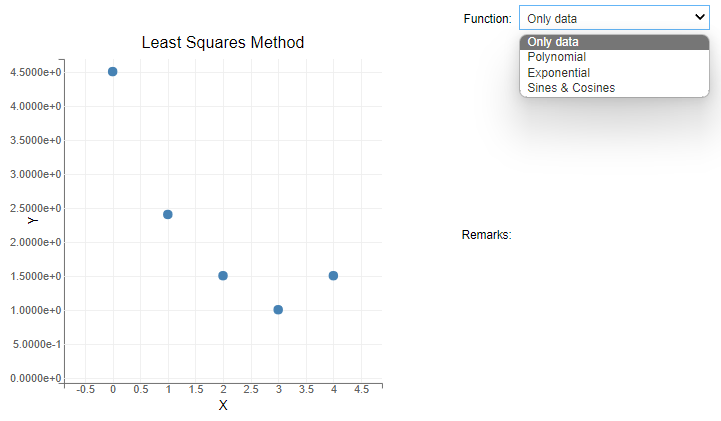
\includegraphics[scale=0.6]{Include/Images/Thesis/Documentation/Visualizers/LeastSquares/Example 1/Example 1 - 00 - Selector.png}
    \item Select Polynomial\\
    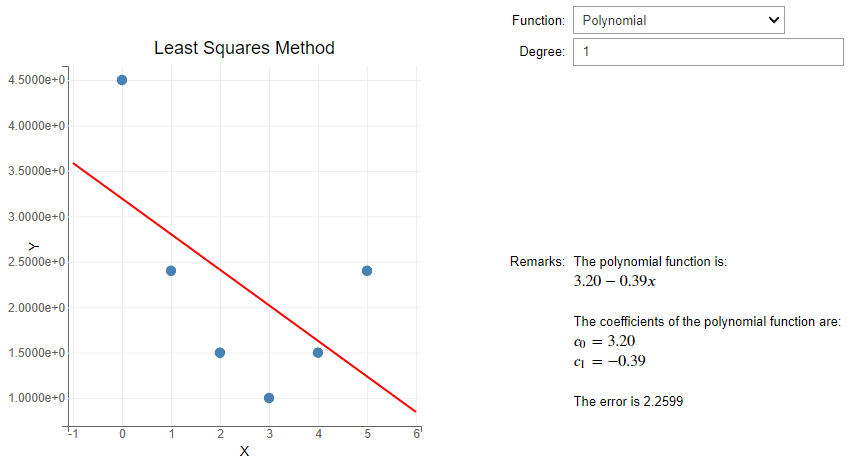
\includegraphics[scale=0.6]{Include/Images/Thesis/Documentation/Visualizers/LeastSquares/Example 1/Example 1 - 00 - Polinomial .png}
    \item Increment degree by 1 (degree 2)\\
    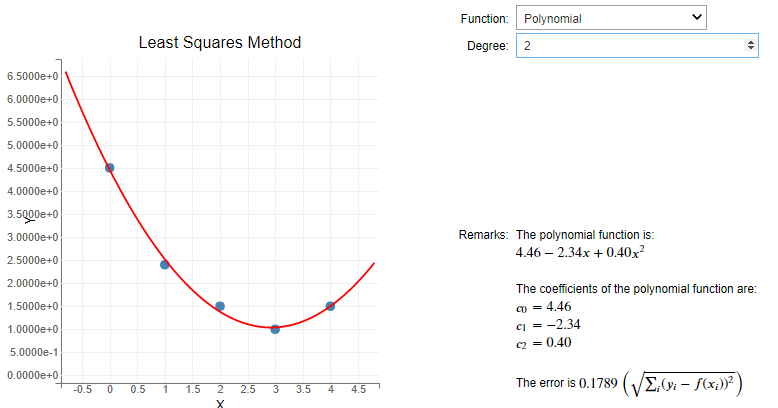
\includegraphics[scale=0.6]{Include/Images/Thesis/Documentation/Visualizers/LeastSquares/Example 1/Example 1 - 01 - Polinomial Degree 2.png}
    \item Degree 5 (Maximum, cannnot go higher)\\
    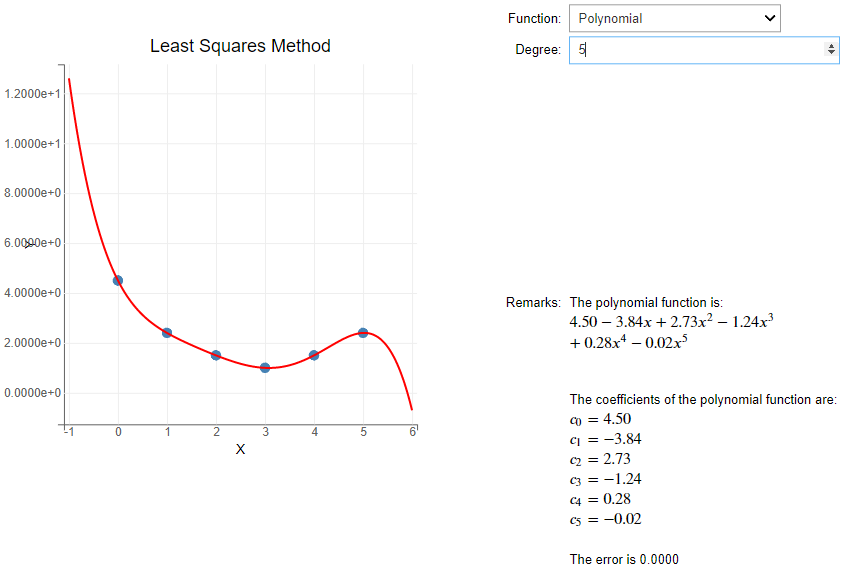
\includegraphics[scale=0.6]{Include/Images/Thesis/Documentation/Visualizers/LeastSquares/Example 1/Example 1 - 02 - Polinomial Degree 5.png}

\end{enumerate}
}

\subsubsection{Example 2: No Input Data and Exponential Fit}
\begin{lstlisting}[language=Python]
from BNumMet.Visualizers.LeastSquaresVisualizer import LSPVisualizer
lspVisualizer = LSPVisualizer()
lspVisualizer.run()
\end{lstlisting}
\begin{enumerate}
    \item Initial state\\
    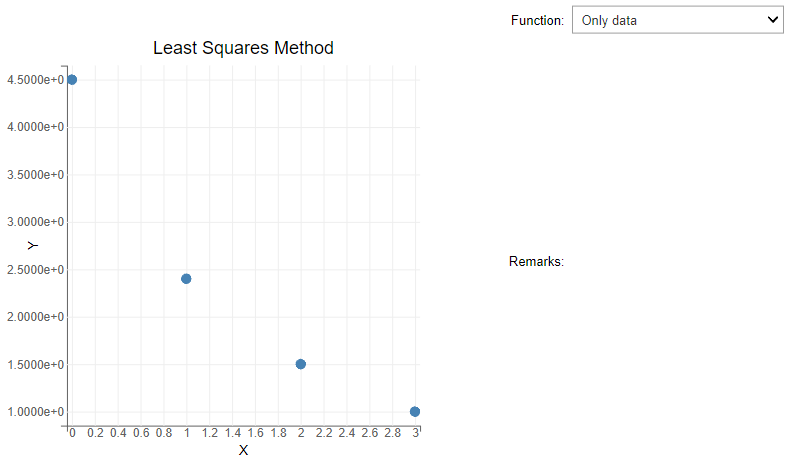
\includegraphics[scale=0.6]{Include/Images/Thesis/Documentation/Visualizers/LeastSquares/Example 2/Example 2 - 00 - Initial State.png}
    \item Exponential Selection\\
    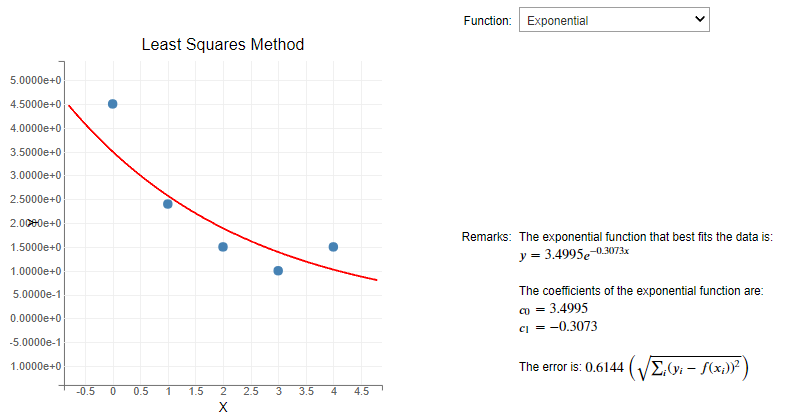
\includegraphics[scale=0.6]{Include/Images/Thesis/Documentation/Visualizers/LeastSquares/Example 2/Example 2 - 00 - Exponential.png}
\end{enumerate}

\subsubsection{Example 3: Sines and Cosines Fit of Varying degree}{
\begin{lstlisting}[language=Python]
from BNumMet.Visualizers.LeastSquaresVisualizer import LSPVisualizer
xData = np.array([0, 1, 2, 3, 4, 5])
yData = np.array([4.5, 2.4, 1.5, 1, 1.5, 2.4])
lspVisualizer = LSPVisualizer(xData, yData)
lspVisualizer.run()
\end{lstlisting}

\begin{enumerate}
    \item Initial State\\
    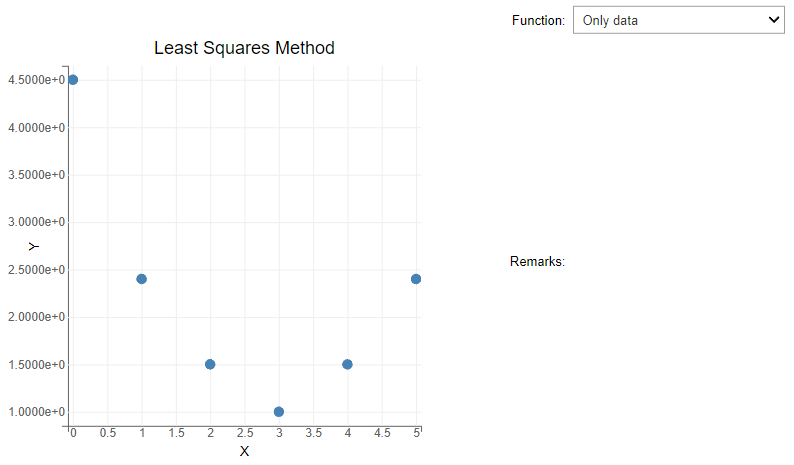
\includegraphics[scale=0.6]{Include/Images/Thesis/Documentation/Visualizers/LeastSquares/Example 1/Example 1 - 00 - Initial State.png}
    \item Selector\\
    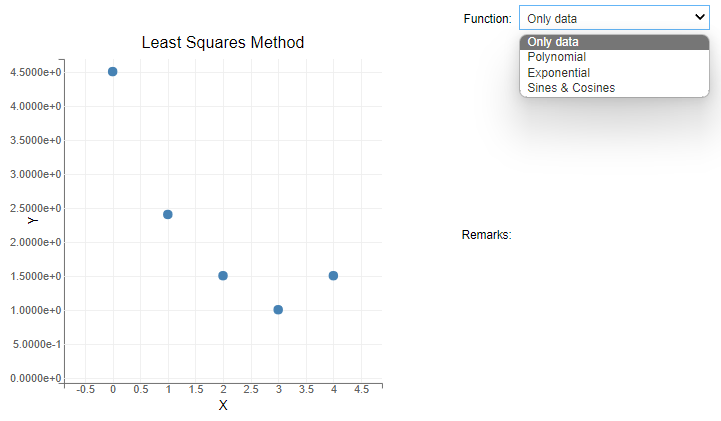
\includegraphics[scale=0.6]{Include/Images/Thesis/Documentation/Visualizers/LeastSquares/Example 1/Example 1 - 00 - Selector.png}
    \item Select Sines \& Cosines\\
    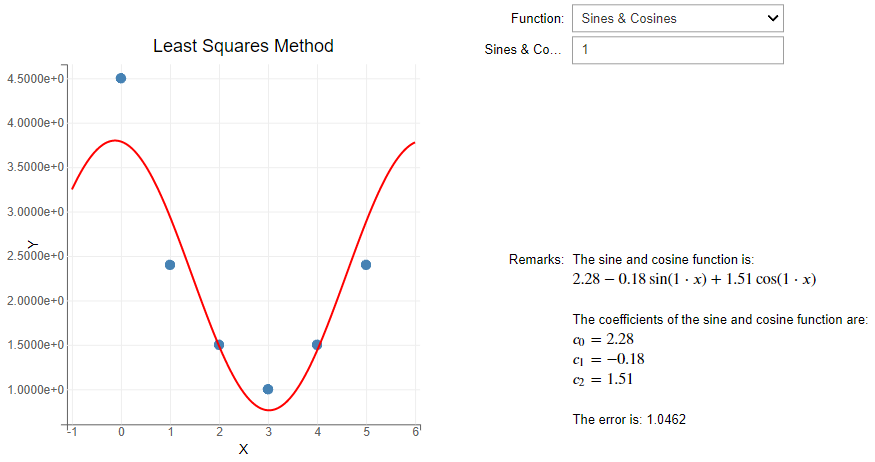
\includegraphics[scale=0.6]{Include/Images/Thesis/Documentation/Visualizers/LeastSquares/Example 3/Example 3 - 00 - Trigonometry.png}
    \item Set degree to the maximum\\
    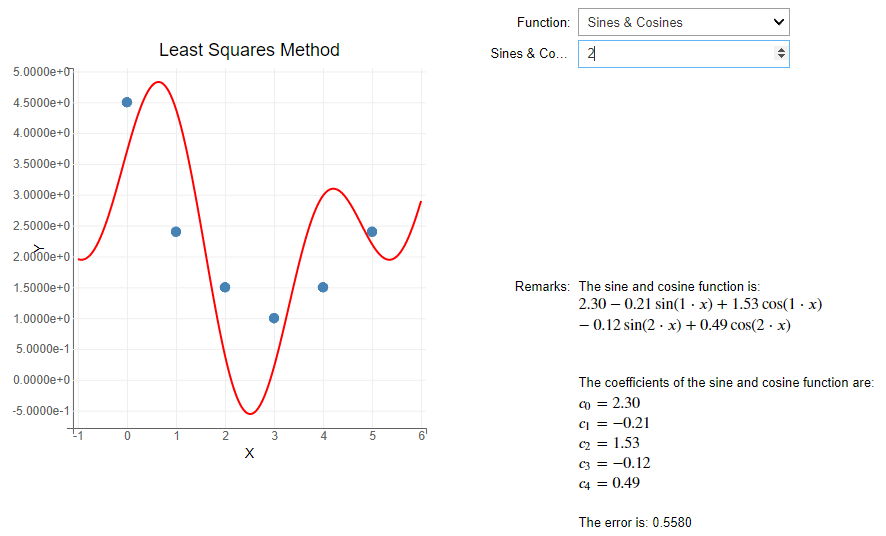
\includegraphics[scale=0.6]{Include/Images/Thesis/Documentation/Visualizers/LeastSquares/Example 3/Example 3 - 01 - Trigonometry Degree 2.png}
\end{enumerate}
}

\subsection{Random Numbers Visualizer}
\subsubsection{Example 1: No input arguments}
\begin{lstlisting}[language=Python]
from BNumMet.Visualizers.RandomVisualizer import RandomVisualizer
randomVisualizer = RandomVisualizer()
randomVisualizer.run()
\end{lstlisting}

\begin{enumerate}
    \item Initial State\\
    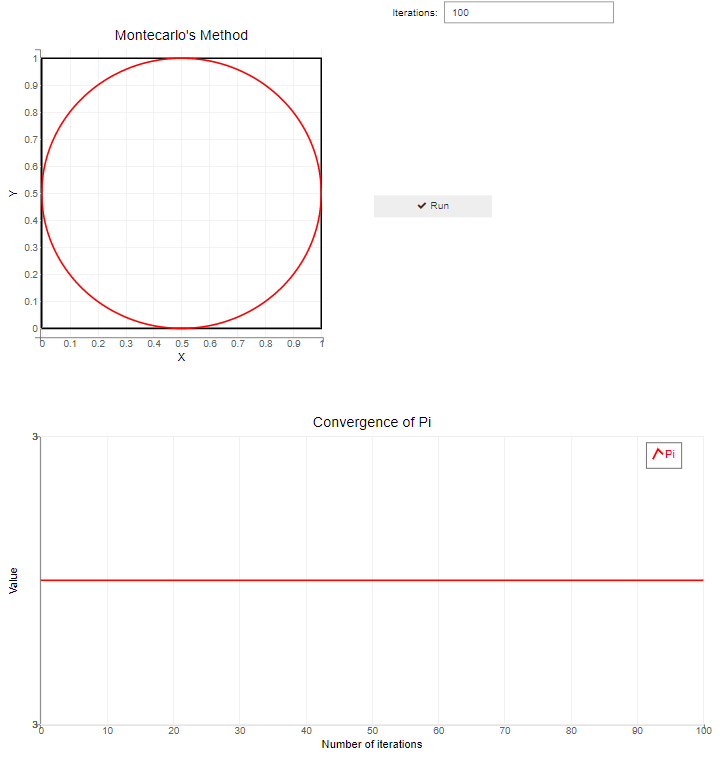
\includegraphics[scale=0.7]{Include/Images/Thesis/Documentation/Visualizers/Randomness/Example 1/Example 1 - 00 - Initial State.png}
    \item Clicked played with 100 default points\\
    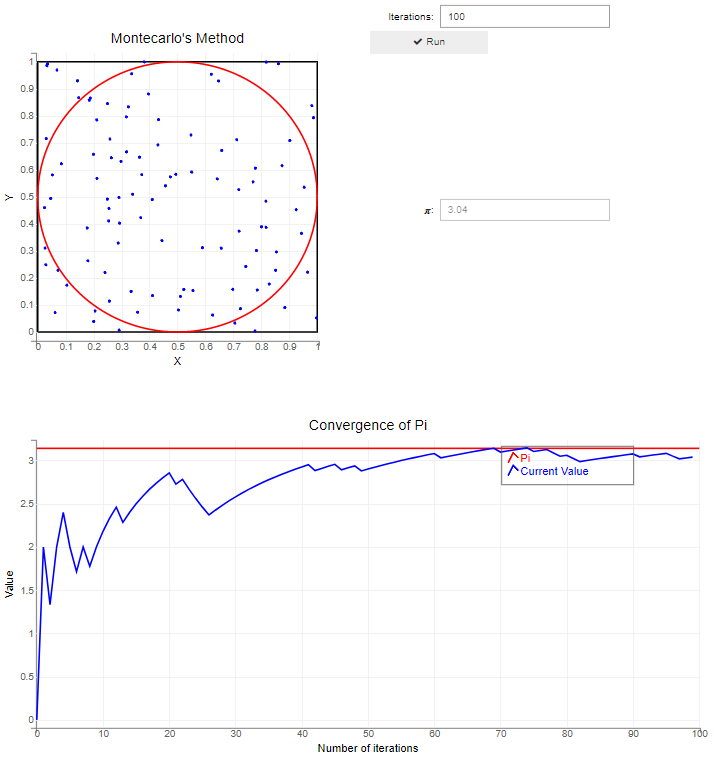
\includegraphics[scale=0.7]{Include/Images/Thesis/Documentation/Visualizers/Randomness/Example 1/Example 1 - 01 - Clicked PLayed.png}
    \item Change number of points to 500 and clicked play\\
    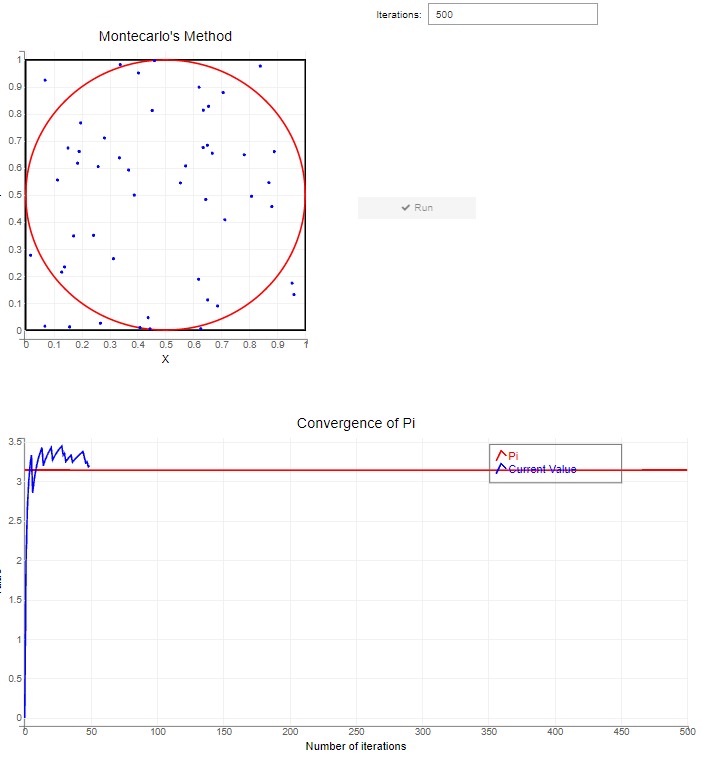
\includegraphics[scale=0.7]{Include/Images/Thesis/Documentation/Visualizers/Randomness/Example 1/Example 1 - 02 - Changed N of points and played.png}
    \item Final of animation playing\\
    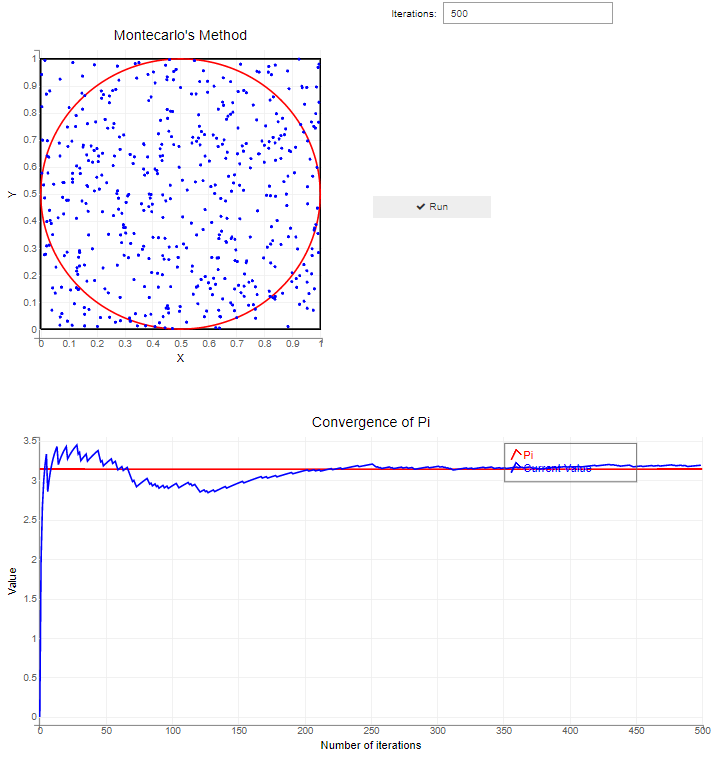
\includegraphics[scale=0.7]{Include/Images/Thesis/Documentation/Visualizers/Randomness/Example 1/Example 1 - 03 - Finished.png}
\end{enumerate}


\subsubsection{Example 2: Input arguments and Ill-Generator}
\begin{lstlisting}[language=Python]
from BNumMet.Visualizers.RandomVisualizer import RandomVisualizer
from BNumMet.Random import marsaglia_rand, clear_marsaglia_vars

clear_marsaglia_vars()
randomFunc = lambda: marsaglia_rand(
    base=10, lag_r=2, lag_s=1, carry=0, seed_tuple=(0, 1)
)
randomVisualizer = RandomVisualizer(randomFunc)
randomVisualizer.run()
\end{lstlisting}

\begin{enumerate}
    \item Initial State\\
    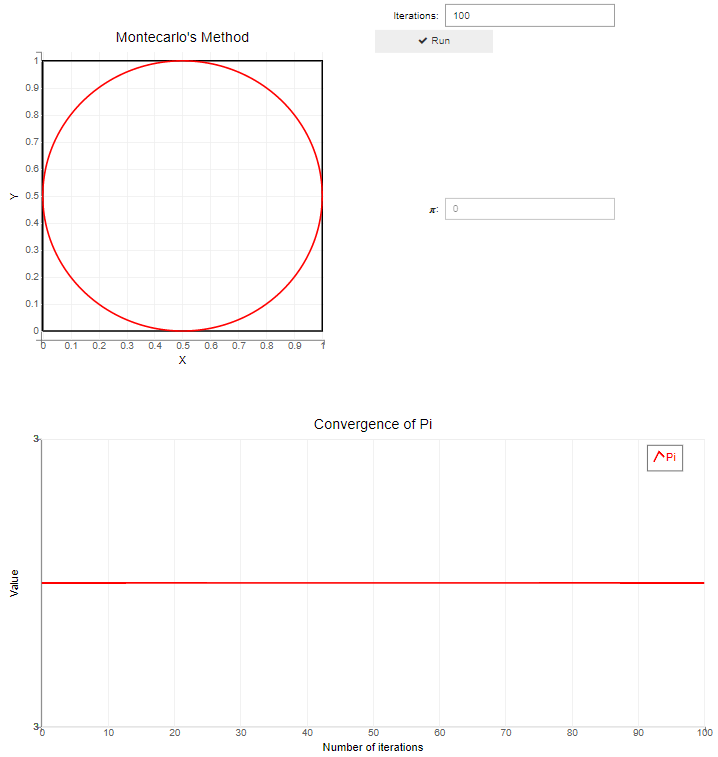
\includegraphics[scale=0.7]{Include/Images/Thesis/Documentation/Visualizers/Randomness/Example 2/Example 2 - 00 - Initial State.png}
    \item Clicked played with 100 default points\\
    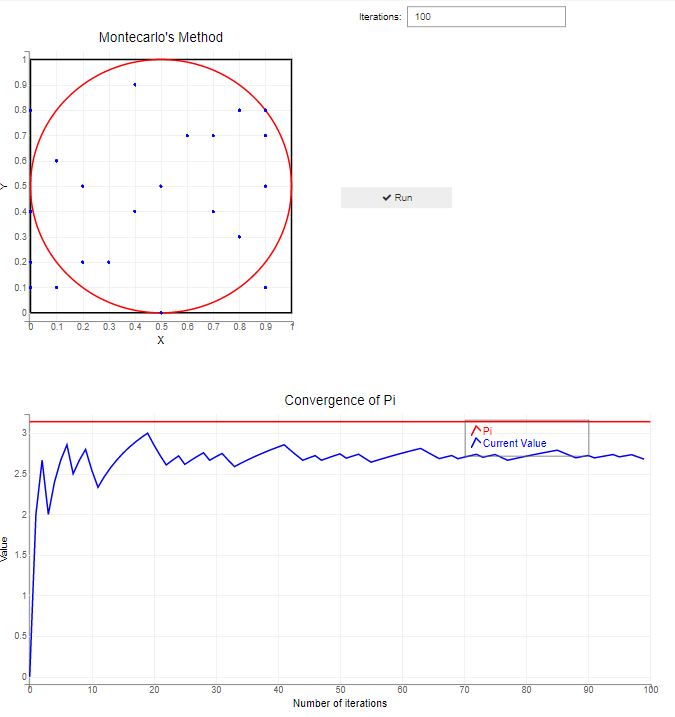
\includegraphics[scale=0.7]{Include/Images/Thesis/Documentation/Visualizers/Randomness/Example 2/Example 2 - 01 - Clicked PLayed.png}
    \item Change number of points to 1000 and clicked play\\
    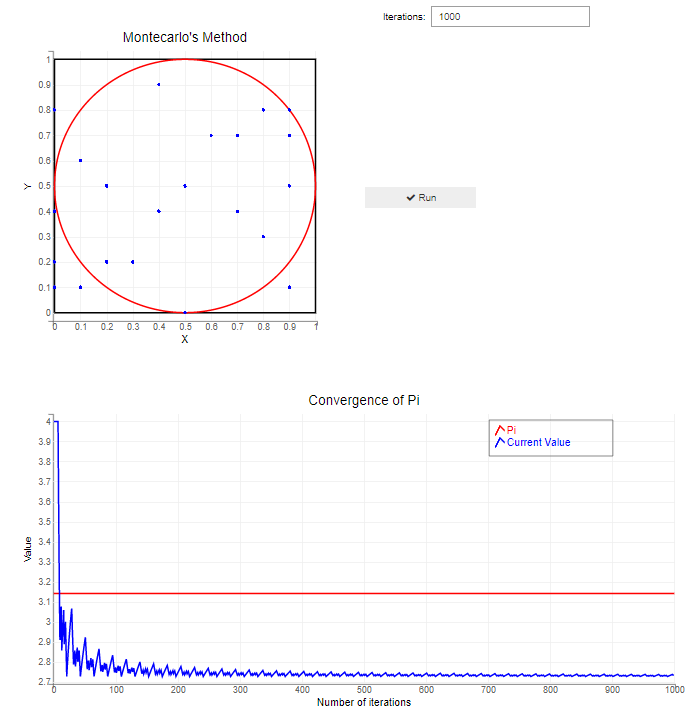
\includegraphics[scale=0.7]{Include/Images/Thesis/Documentation/Visualizers/Randomness/Example 2/Example 2 - 02 - 1000 points played.png}

\end{enumerate}
